\documentclass{beamer}
\usepackage[T1]{fontenc}
\usepackage{lmodern}

\mode<presentation>
\usetheme[footline=empty]{Magicc}

\usepackage{graphicx}
\graphicspath{{figures/}}
\DeclareGraphicsExtensions{.pdf, .png, .jpg}

\usepackage{tikz}

% add logo to slide header
\addtobeamertemplate{frametitle}{}{%
\begin{tikzpicture}[remember picture,overlay]
\node[anchor=north east,yshift=2pt] at (current page.north east) {
\includegraphics[height=0.75cm]{logo_white}};
\end{tikzpicture}}

% create outline slide at each \section{} (optional)
\AtBeginSection[]{\frame{\frametitle{Outline}\tableofcontents[currentsection]}}

% presentation info
\title{Multi-dimensional Optimization of Gasoline-fueled Variable Pitch Multirotor Aircraft}
%\title[Short Title]{GAS Quad}
\author{Dallin Briggs, Gary Ellingson}
\institute[MAGICC Lab]{
\includegraphics[height=0.5in]{logo_gray}}
\date{\today}

\begin{document}

\begin{frame}
\titlepage
\end{frame}

\begin{frame}{Presentation Guidelines}

You will sign up for a 10 minute presentation time slot. The presentation is graded only for completion. Group projects will have 8 minutes to present and 2 minutes for Q\&A. Individuals will have 6 minutes to present and 2 minutes for Q\&A. Obviously you will not have a lot of time to spend on details. Instead, you should focus on motivation (what the problem is and why it is important), the solution approach, and the most important results. Each member of the team should have a role in the presentation.

\end{frame}

\begin{frame}{Outline}
\begin{itemize}
	\item{Motivation and Background}
	\item{---figure of multirotor trends in flight time}
	\item{---focus on OTS stuff bases our design on empirical models}
	
	\item{Theory - models}
	\item{---Engine model}
	\item{---Aero model}
	
	\item{Optimization}
	\item{---Objective only directly a function of 2 design variables}
	\item{---constraints}
	
	\item{Results}
	\item{lessons learned}
	\item{questions}
\end{itemize}
\end{frame}

\begin{frame}{Motivation and Background}
	\begin{center}
	Currently available multirotor capabilities
	\end{center}
	\begin{figure}
		\begin{center}
			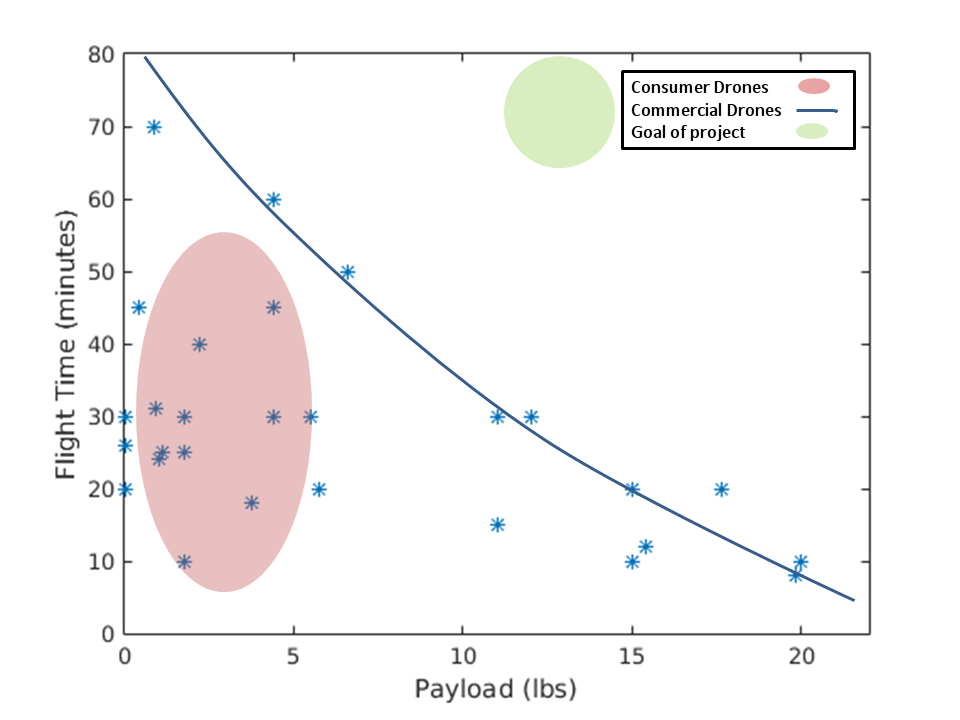
\includegraphics[width=.70\textwidth]{current_rev.png}
			\label{current_capabilities}
		\end{center}
	\end{figure}
\end{frame}

\begin{frame}{Engine Models}

	\begin{figure}
		\begin{center}
			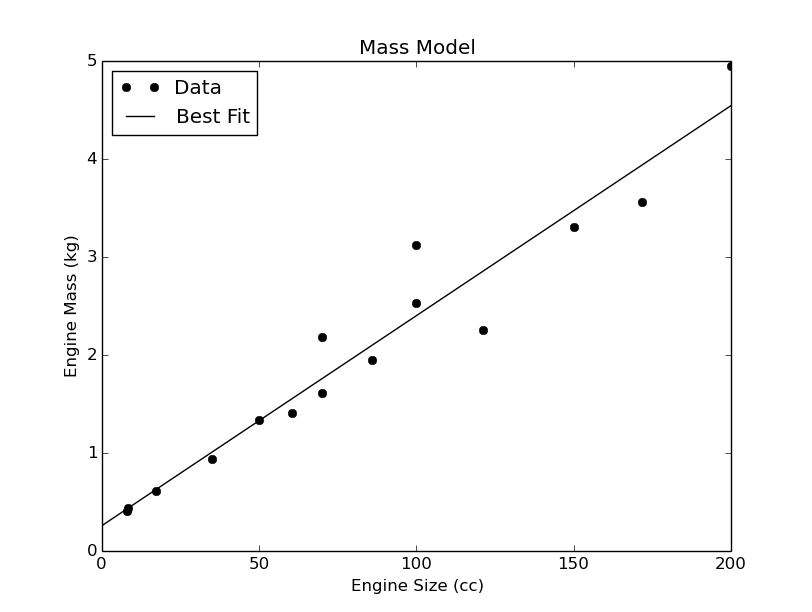
\includegraphics[width=.70\textwidth]{../mass.png}
			\label{fig:eng_mass}
		\end{center}
	\end{figure}
\end{frame}

\begin{frame}{Engine Models}	
	\begin{figure}
		\begin{center}
			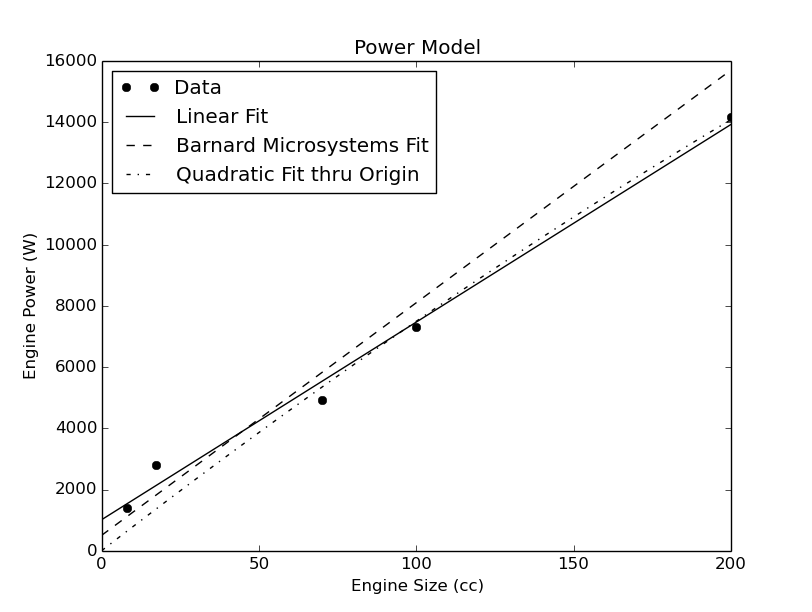
\includegraphics[width=.70\textwidth]{../max_power.png}
			\label{fig:eng_power}
		\end{center}
	\end{figure}
	
\end{frame}

\begin{frame}{Models}
	\begin{itemize}
		\item{To represent the aerodynamics of each rotor, we used Combined Differential Blade Element and Momentum Theory for nonuniform inflow.}
		\begin{center}
		$ dT = \frac{1}{2} \rho a \Omega^2 r^2 (\theta - \phi) c \  dr $
		
		$ dQ = \frac{1}{2} \rho \Omega^2 r^3 c (\delta + \phi C_L) \ dr $
		\end{center}
	\end{itemize}

\end{frame}

\begin{frame}{Optimization Method}

\end{frame}

\begin{frame}{Results}

\end{frame}

\begin{frame}{Lessons Learned}

\end{frame}

\begin{frame}{Questions}

\end{frame}

\end{document}

